\documentclass{beamer}

\mode<presentation> {
\usetheme{Madrid}
}

\usepackage{graphicx}
\usepackage{svg}
\usepackage{booktabs}
\usepackage{amsmath}
\usepackage[T1]{fontenc}
\usepackage[french]{babel}
\usepackage{url,color}
\usepackage{subfigure}
\usepackage{amsthm,amsfonts,amssymb,amscd,amsxtra, multicol}
\usepackage{comment}

\graphicspath{ {./images/} }

\title{Conception d'un SaaS pour les cours en ligne en milieu universitaire}
\author[Hans TOGNON]{Hans B. K. \textbf{TOGNON} \\ Supervisé par Ing. Miranda \textbf{GNONLONFOUN}}
\institute[IFRI]{
\textbf{I}nstitut de \textbf{F}ormation et de \textbf{R}echerche en  \textbf{I}nformatique \\
\medskip
\textbf{\color{purple}\href{mailto:contact@ifri.uac.bj}{contact@ifri.uac.bj}}
}

\begin{document}
% %%%%%%%%%%%%%%%%%%%%%%%%%%%%%%%%%%
% Title Page
% %%%%%%%%%%%%%%%%%%%%%%%%%%%%%%%%%%
\begin{frame}
  \thispagestyle{empty}
  \begin{multicols}{2}
    \begin{figure}
        \flushleft
        
\includegraphics[width=0.11\textwidth]{logoifri}
    \end{figure}
    \begin{figure}
        \flushright
        
\includegraphics[width=0.1\textwidth]{logouac}
    \end{figure}
    \end{multicols}
    \vspace{-1cm}
  \titlepage
  \end{frame}

% %%%%%%%%%%%%%%%%%%%%%%%%%%%%%%%%%%
% ToC
% %%%%%%%%%%%%%%%%%%%%%%%%%%%%%%%%%%
\begin{frame}
  \frametitle{PLAN}
  \begin{itemize}
    \item Introduction
    \item Revue de Littérature
    \item Matériels et méthodes
    \item Résultats \& Discussion
    \item Conclusion \& Perspectives
  \end{itemize}
\end{frame}

% %%%%%%%%%%%%%%%%%%%%%%%%%%%%%%%%%%
% Introduction
% %%%%%%%%%%%%%%%%%%%%%%%%%%%%%%%%%%
\begin{frame}{Introduction}
  \begin{block}{Contexte}
    L'expansion du numérique dans le milieu éducatif, aujourd'hui, est un fait.
    Des situations tels la récente pandémie de COVID-19 ou encore le manque de cadres
    de cours adéquats rendent le besoin encore plus d'actualité. Ceci requiert également un
    certain investissement de la part des divers acteurs du milieu.
  \end{block}

  \begin{block}{Problématique}
    Comment mettre en place une application pour répondre au besoin relatifs aux
    cours en ligne, tout en éliminant les barrières d'ordres logistique et financier 
    imposées par les solutions génériques, afin de recréer un environnement de classe virtuel?
  \end{block}
\end{frame}

\begin{frame}{Introduction}
  \begin{block}{Objectifs}
    Concevoir un prototype d'application pour tenir les cours en ligne:
    \begin{itemize}
      \item organiser les entités en sections bien définies ;
      \item définir le calendrier des cours à tenir ;
      \item organiser des sessions d’audio-conférence pour le déroulement des cours ;
      \item implémenter des fonctionnalités annexes pour une bonne expérience utilisateur ;
      \item minimiser certains coûts liés à l'exploitation d'une telle solution.
    \end{itemize}
  \end{block}
\end{frame}

% %%%%%%%%%%%%%%%%%%%%%%%%%%%%%%%%%%
% Revue de Littérature
% %%%%%%%%%%%%%%%%%%%%%%%%%%%%%%%%%%
\begin{frame}{Revue de Littérature : \small{Termes}}
  \begin{block}{Formation à distance}
    Forme d’enseignement ou l’enseignant et l’étudiant sont séparés dans le temps et/ou par l’espace.
    Les cours en ligne en sont la dérivée la plus exploitée.
  \end{block}
  \begin{block}{WebRTC}
    \textit{Web Real-Time Communication}. Il s'agit d'un protocole activement exploité dans la mise en oeuvre
    d'application de communication en temps réel.
  \end{block}
  \begin{block}{SaaS}
    \textit{Software as a Service}. Il s'agit d'un modèle de distribution logicielle.
  \end{block}
\end{frame}

\begin{frame}{Revue de Littérature : \small{Solutions existantes}}
  \begin{block}{Solutions}
    \begin{itemize}
      \item Google Classrooms/Google meet
      \item Zoom
      \item Moodle/BigBlueButton
    \end{itemize}
  \end{block}
  \begin{block}{Limites}
    \begin{itemize}
      \item Modèles de souscription basé sur le nombre d'utilisateurs et parfois complexes
      \item Prise en main technique requise
      \item Consommation large de données
    \end{itemize}
  \end{block}
\end{frame}
% %%%%%%%%%%%%%%%%%%%%%%%%%%%%%%%%%%
% Matériels et méthodes
% %%%%%%%%%%%%%%%%%%%%%%%%%%%%%%%%%%
\begin{frame}{Matériels et Méthodes : \small{UML} - \footnotesize{Diagramme de cas d'utilisation}}
  \begin{figure}[H]
    \centering
    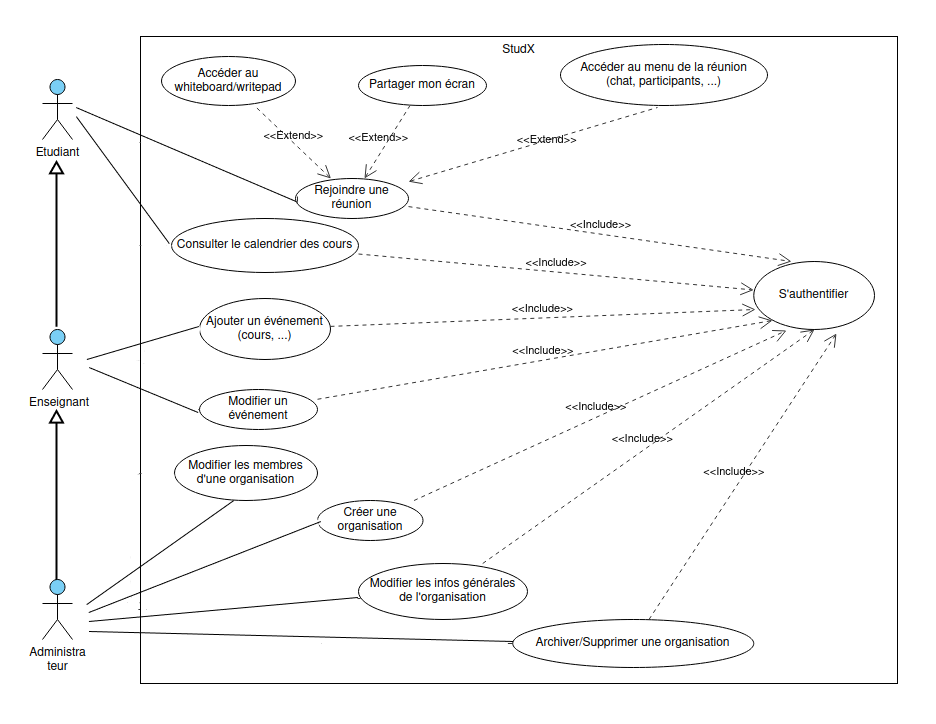
\includegraphics[width=\textwidth]{../../images/use-cases-diag.png}
    \caption{Cas d'utilisation}
\end{figure}
\end{frame}

\begin{frame}{Matériels et Méthodes : \small{UML} - \footnotesize{Diagramme de classe}}
  \begin{figure}[H]
    \centering
    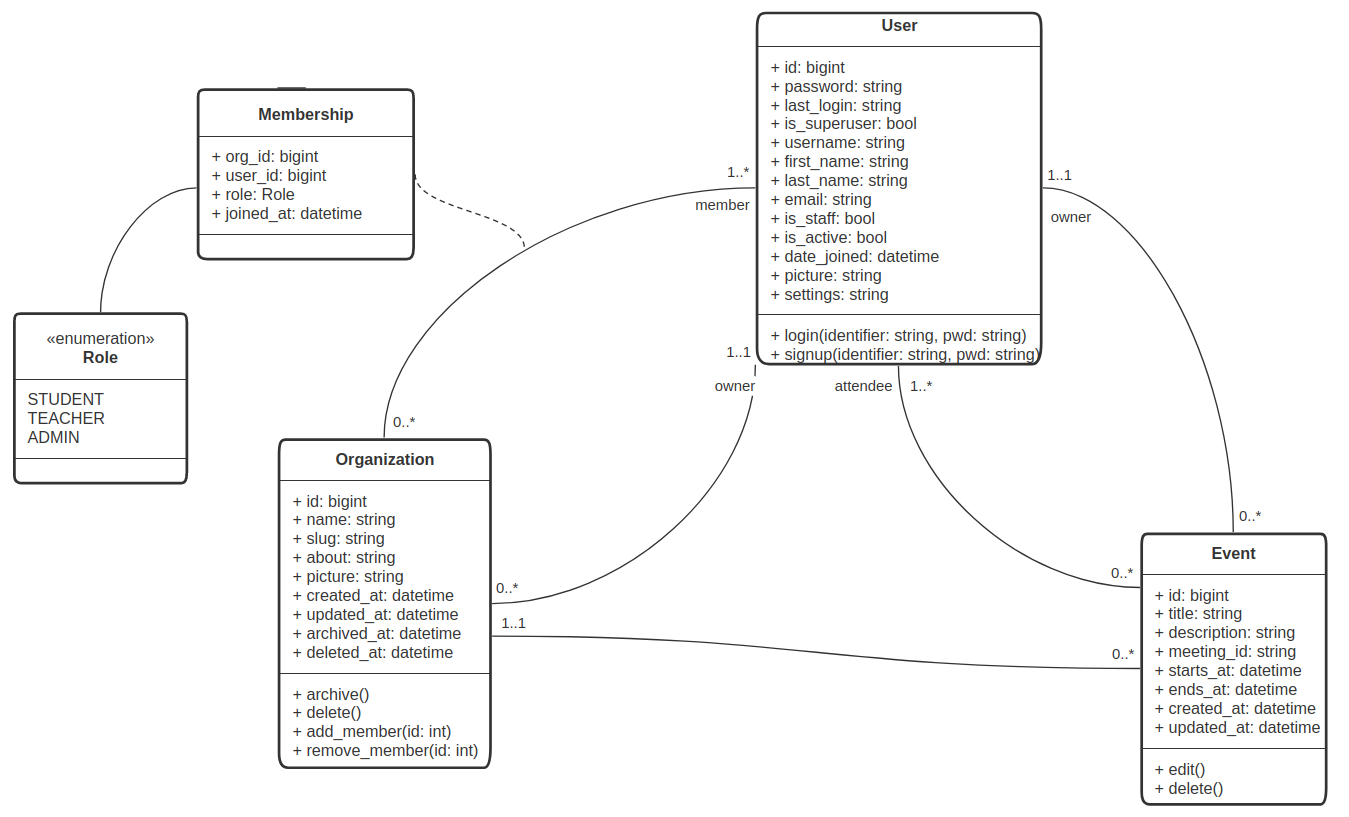
\includegraphics[width=\textwidth]{../../images/class-diag.png}
    % \caption{Diagramme de classe}
\end{figure}
\end{frame}

\begin{frame}{Matériels et Méthodes : \small{UML} - \footnotesize{Diagramme de séquence}}
  \begin{figure}[H]
    \centering
    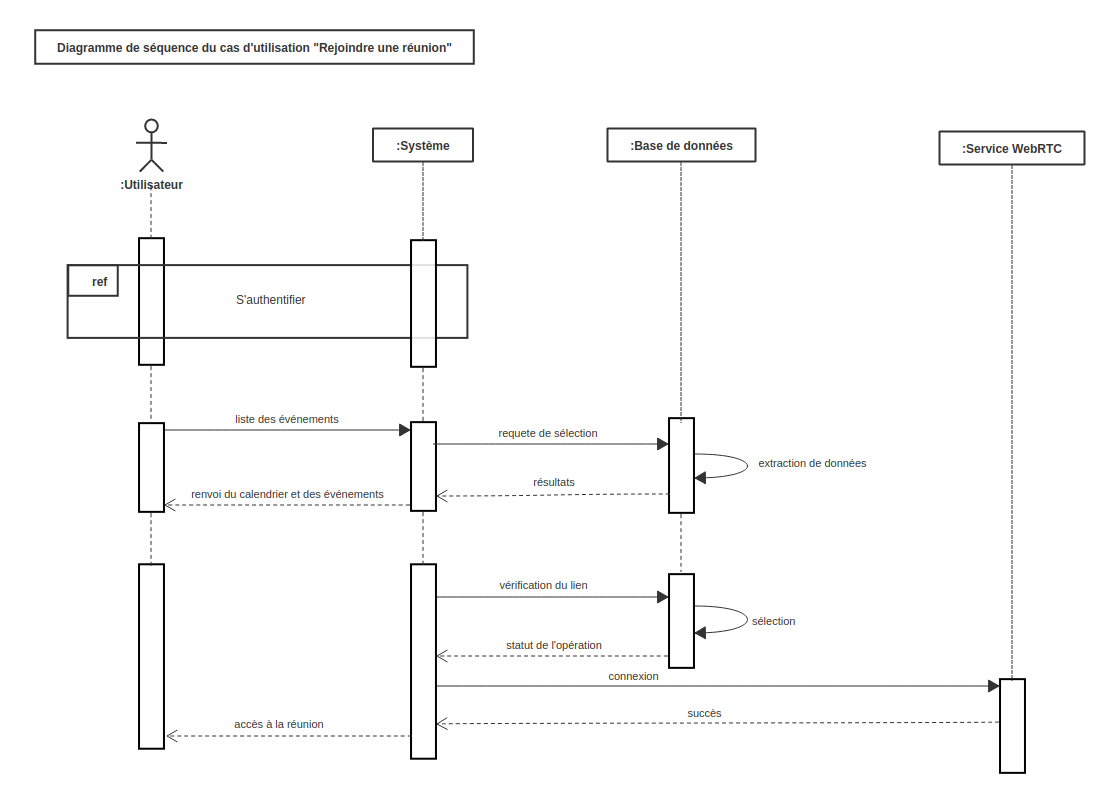
\includegraphics[width=0.9\textwidth]{../../images/join-meet-sequence-diag.png}
    % \caption{Diagramme de séquence (fonctionnalité principale)}
\end{figure}
\end{frame}

\begin{frame}{Matériels et Méthodes : \small{Technologies}}
  \begin{figure}[H]
    \centering
    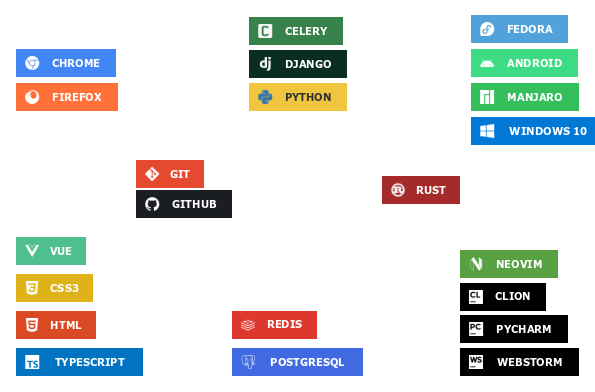
\includegraphics[width=0.9\textwidth]{tools}
    % \caption{Outils technologiques}
\end{figure}
\end{frame}


% %%%%%%%%%%%%%%%%%%%%%%%%%%%%%%%%%%
% Résultats et Discussion
% %%%%%%%%%%%%%%%%%%%%%%%%%%%%%%%%%%
\begin{frame}{Résultats \& Discussion}
  \begin{center}
    \Huge{Démonstration !}
  \end{center}
\end{frame}

\begin{frame}{Résultats \& Discussion}
  \begin{block}{}
    La mise en place du prototype a nécéssité la mise en place et la coordination de plusieurs technologies.
    Les fonctionnalités prévues ont été implémentées. Deployée à grande échelle dans un réseau local, elle permet un usage en mode totalement non connecté.
  \end{block}

  \begin{block}{Code source}
    Le code source de l'application est disponible à l'adresse suivante:
    \url{https://github.com/tobihans/studx.git}.
  \end{block}
\end{frame}

\begin{frame}{Résultats \& Discussion}
  \begin{block}{Difficultés}
    \begin{itemize}
      \item WebRTC est une technologie relativement nouvelle bien que fréquemment employée ;
      \item Il s'agit d'une technologie complexe à prendre en main ;
      \item Bogues natifs liés aux navigateurs exploités (exemple: \url{https://bugs.chromium.org/p/chromium/issues/detail?id=933677})
    \end{itemize}
  \end{block}
\end{frame}

% %%%%%%%%%%%%%%%%%%%%%%%%%%%%%%%%%%
% Conclusion et Perspectives
% %%%%%%%%%%%%%%%%%%%%%%%%%%%%%%%%%%
\begin{frame}{Conclusion \& Perspectives}
  \begin{block}{}
    Le projet développé fournit un cadre moderne de communication 
    en temps réel pour l'apprentissage virtuel, avec la possibilité d'étendre ses fonctions à l'avenir;
    ceci, tout en réduisant les coûts pour les utilisateurs.
  \end{block}

  \begin{block}{Perspectives}
    \begin{itemize}
      \item Enregistrer les sessions pour un usage ultérieur ;
      \item Sauvagarder l'historique de la messagerie instantannée
      \item Intégrer un modèle Machine Learning pour le traitement du signa audio et sa conversion
      en langage des signes.
    \end{itemize}
  \end{block}
\end{frame}

% Thanks
\begin{frame}
  \begin{center}
  \Huge{Merci !}
  \end{center}

\end{frame}

\end{document}
